% =========================================================================== %

\begin{frame}[t,plain]
\titlepage
\end{frame}

% =========================================================================== %

\begin{frame}{Efficiency}
%
\begin{center}
	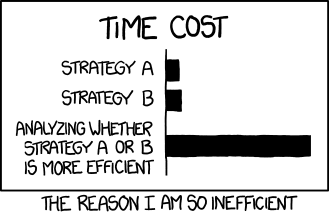
\includegraphics[width=.4\linewidth]{./gfx/xkcd-efficiency}\\
	\emph{I need an extension for my research project because I spent all month trying to figure out whether learning Dvorak would help me type it faster.}

	\vspace{6pt}
	Source: \url{https://xkcd.com/1445/}
\end{center}
%
\end{frame}

% =========================================================================== %

\begin{frame}{What does Efficiency Mean?}
%
\begin{itemize}
\item Time Efficiency
	\begin{itemize}
	\item Idea: How fast does code do its job
	\item Scalability: If I put twice as much data into the code, how much longer does it take
	\end{itemize}
\item Memory Efficiency
	\begin{itemize}
	\item Idea: How much memory is used to compute the result
	\item Also: differentiate between absolute requirement and scaling behaviour
	\end{itemize}
\item Devellopment Efficiency
	\begin{itemize}
	\item Idea: How often is this code useful?
	\item How many input scenarios can be dealt with?
	\item How much \enquote{machinery} is needed to use the result?
	\item How much machinery is needed to prepare the input?
	\end{itemize}
\end{itemize}
%
\end{frame}

% =========================================================================== %

\begin{frame}[fragile]{Time Efficiency}
%
\begin{columns}[T]
\column{.5\linewidth}
\begin{itemize}
\item To write fast code, we need to recognize fast code
\item Measure directly
	\begin{itemize}
	\item Function \texttt{time.time}: Time in seconds since some \emph{epoch}
	\item Millisecond resolution
	\item Improve Accuracy by measuring repeated execution
	\end{itemize}
\item Count instructions
\begin{itemize}
\item Idea of FLOPs: \emph{floating point operations}
\item Assumption: All FLOPs take the same time (approximately true)
\item Loops: Multiplication
\item Nested Loops: Exponentiation
\end{itemize}
\end{itemize}
%
\column{.5\linewidth}
\begin{codebox}[Scheme: Time Requirement]
\begin{minted}[linenos, fontsize=\scriptsize]{python3}
import time

R = 1000

tic = time.time()
for run in range(R) :
    # algorithm
toc = time.time()

print(f"it took {toc - tic} second to "
      f"run the algorithm {R} times")
\end{minted}
\end{codebox}

\end{columns}
%
\end{frame}

% =========================================================================== %

\begin{frame}[fragile]
%
\begin{columns}[T]
\column{.5\linewidth}
\begin{Large}
	{Counting Instructions}
	\vspace{6pt}
\end{Large}
%
\begin{itemize}
\item Notation: \inPy{N = len(data)}
\item Most Algorithms: Conditions
\item Implicit Assumptions: best / worst / average case
\item Best case
	\begin{itemize}
	\item \texttt{data} is such that \inPy{if} condition is \inPy{False} most of the time
	\item 2 assignments before the loop
	\item 2 assigments per iteration (\texttt{i}, \texttt{x})
	\item $N$ comparisons
	\item 0 assignments in the loop
	\item[\Thus] $4 + N$ FLOPs
	\end{itemize}
\end{itemize}
%
\column{.5\linewidth}
\begin{codebox}[Example: Find Minimum]
\begin{minted}[fontsize=\scriptsize]{python3}
data = [...]

def findMin(data) :
    theMin = data[0]
    idxMin = 0
    for i, x in enumerate(data) :
        if theMin > x :
            idxMin = i
            theMin = x
    return theMin, idxMin
\end{minted}
\end{codebox}
%
\begin{itemize}
\item Worst case
	\begin{itemize}
	\item Enter \inPy{if} block every time
	\item 2 assignments per loop
	\item[\Thus] $4 + 3N$ FLOPs
	\end{itemize}
\end{itemize}
\end{columns}
%
\end{frame}

% =========================================================================== %

\begin{frame}[fragile]{Counting Instructions}
%
\begin{columns}[T]
\column{.5\linewidth}
\begin{itemize}
\item Nested Loops
\item Somewhat \enquote{hidden}
\item One multiplication per inner \inPy{list} element
\item \texttt{columns} inner \inPy{list} elements
\item \texttt{rows} inner \inPy{list}s
\item[\Thus] $\texttt{rows} \cdot \texttt{columns}$ FLOPs
\item Often: only one size Parameter $N$
	\begin{itemize}
	\item \ie here: \texttt{rows == columns}
	\item[\Thus] $N^2$ FLOPs
	\end{itemize}
\end{itemize}
%
\column{.5\linewidth}
\begin{codebox}[Example: Generate Table]
\begin{minted}[fontsize=\scriptsize]{python3}
productTable = [
    [r * c 
     for c in range(1, columns + 1)
    ] for r in range(1, rows + 1)
]
\end{minted}
\end{codebox}
%
\begin{itemize}
\item An exact evaluation requires somewhat deep knowledge of the internal structures in play.
\item How many FLOPs might \inPy{print(list)} take?
\end{itemize}
\end{columns}
%
\end{frame}

% =========================================================================== %

\begin{frame}{Scaling Behaviour and Asymptotic Time Complexity}
%
\begin{columns}[T]
\column{.5\linewidth}
\begin{itemize}
\item Previous Considerations based on assumption: all FLOPs take same time
\item Only approximately true
\item Still: Useful for comparing algorithms
\item But: Don't take the numbers too seriously
\item Instead: \enquote{grand picture}
\item Which is faster?
	\begin{itemize}
	\item $T_1(N) = 6N + 20$
	\item $T_2(N) = 2N^2$
	\end{itemize}
\item $T_2$ starts out superior, but soon is outclassed by $T_1$
\end{itemize}
%
\column{.5\linewidth}
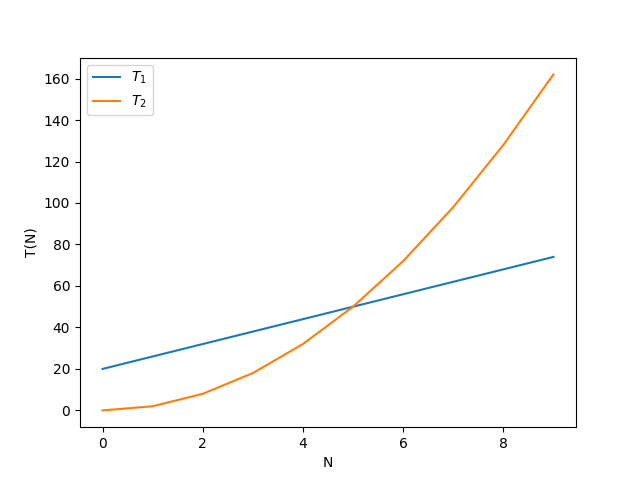
\includegraphics[width=\linewidth]{./gfx/linearVsQuadratic}
We usually are interested in the behaviour for big $N$
\end{columns}
%
\end{frame}

% =========================================================================== %

\begin{frame}{Asymptotic Time Complexity and Landau Notation}
%
\begin{columns}[T]
\column{.5\linewidth}
\begin{itemize}
\item For big $N$, the highest power always \enquote{wins}
\item Even prefactors are not important for $N \thus \infty$
\item Landau Notation or Big O Notation
	\begin{itemize}
	\item Imprecisely: highest order term
	\item Mathematical definition:
	\begin{align*}
		f(x) \in \mathcal{O}(g(x))
		~
		\Leftrightarrow
		~
		\limsup_{x \to \infty} 
			\frac
			{|f(x)|}
			{g(x)}
		< \infty
	\end{align*}
	\item $\Theta(f(N)), \Omega(f(N))$ (imprecisely): Upper/lower bound of growth rate
	\end{itemize}
\end{itemize}
%
\column{.5\linewidth}
\begin{itemize}
\item $\mathcal{O}(1)$ (\emph{constant time}) is faster than
\item $\mathcal{O}(\log(N))$ (\emph{logarithmic time}) is faster than
\item $\mathcal{O}(N^{\alpha})$ (\emph{polynomial time}) for any $\alpha > 0$ is faster than
\item $\mathcal{O}(N^{\alpha} \log(N))$ is faster than
\item $\mathcal{O}(N^{\beta})$ for any $\beta > \alpha$ is faster than
\item $\mathcal{O}(\exp(N))$ (\emph{exponential time}) is faster than
\item $\mathcal{O}(N^N)$ or $\mathcal{O}(N!)$ is faster than ...
\end{itemize}
\end{columns}
%
\end{frame}

% =========================================================================== %

\begin{frame}[fragile]
%
\begin{columns}[T]
\column{.5\linewidth}
\begin{Large}
	{Time Complexity and Recursion}
	\vspace{6pt}
\end{Large}
%
\begin{itemize}
\item Remember binary search: recursively reduce list length
\item $\mathcal{O}(\log(N))$
\item Time complexity hard to \enquote{count}
\item Master Theorem
	\begin{itemize}
	\item $T(N) = a T(\frac{N}{b}) + f(N)$
	\item $a$: number of recursion calls (here: 1)
	\item $b$: data reduction factor (here: 2)
	\item $f$: overhead (here: $f \in \mathcal{O}(1)$)
	\end{itemize}
\item Depending on $a, b, f$: three cases
\item Note: not applicable for \emph{all} recursive algorithms
\end{itemize}
%
\column{.5\linewidth}
\begin{codebox}[Example: Binary Search]
\begin{minted}[linenos, fontsize=\scriptsize]{python3}
data = [...].sort()

def binarySearch (data, searchTerm) :
  size = len(data)
  if (size == 1) :
    if data[0] == searchTerm :
      return True
    else                     :
      return False
  else :
    midPoint = size // 2
    if   data[midPoint] == searchTerm :
      return True
    elif data[midPoint]  < searchTerm :
      return binarySearch(
        data[midPoint:], searchTerm)
    else                              :
      return binarySearch(
        data[:midPoint], searchTerm)
\end{minted}
\end{codebox}
\end{columns}
%
\end{frame}

% =========================================================================== %

\begin{frame}{Master Theorem}
%
\begin{itemize}
\item $T(N) = a T(\frac{N}{b}) + f(N)$
\item $c_{\text{crit}} \coloneqq \log_b(a)$
\item Case 1: \emph{leaf-heavy}: subproblems dominate
	\begin{itemize}
	\item $f \in \mathcal{O}(N^c)$ for a $c < c_{\text{crit}}$
	\item[\Thus] $T \in \Theta(N^{c_{\text{crit}}})$
	\end{itemize}
\item Case 2: \emph{trunk-heavy}: overhead and subproblems comparable in effort
	\begin{itemize}
	\item $f \in \Theta(N^{c_{\text{crit}}} \log^k(N))$ for some $k$
	\item[\Thus] $T \in \Theta(N^{c_{\text{crit}}} \log^{k+1}(N) )$
	\end{itemize}
\item Case 3: \emph{root-heavy}: work to split/recombine dominates
	\begin{itemize}
	\item $f \in \Omega(N^c)$ for a $c > c_{\text{crit}}$
	\item $af(\frac{N}{b}) \leq kf(N)$ for some $k < 1$ (\emph{regularity condition})
	\item[\Thus] $T \in \Theta(f(N))$
	\end{itemize}
\end{itemize}
%
\end{frame}

% =========================================================================== %

\begin{frame}[fragile]{Lazy Evaluation}
%
\begin{itemize}
\item Consider \inPy{if someFunc() and otherFunc() : ...}
\item if \texttt{someFunc()} was already evaluated to \inPy{False}, we don't need to evaluate \texttt{otherFunc}
\item Principle:
	\begin{minted}[linenos, fontsize=\scriptsize]{python3}
if someFunc() :
    if otherFunc() :
        ...
	\end{minted}
\item Actually, Python does this automatically for logical operators (\thus \emph{Short Circuiting})
\item[\Thus] Put the easy to evaluate expression first!
\end{itemize}
%
\end{frame}

% =========================================================================== %

\begin{frame}[fragile]{Takeaway: How Do We Write Fast Code?}
%
\begin{columns}[T]
\column{.5\linewidth}
\begin{itemize}
\item Have a look at your loops!
\item What is computed repeatedly?
	\begin{itemize}
	\item Bad:
	\begin{minted}[linenos, fontsize=\scriptsize]{python3}
data = [...]
for i in range(len(data)) :
    data[i] /= len(data)
	\end{minted}
	
	\item Better:
	\begin{minted}[linenos, fontsize=\scriptsize]{python3}
data = [...]
f = len(data)
for i in range(f) :
    data[i] /= f
	\end{minted}
	
	\end{itemize}
\end{itemize}
%
\column{.5\linewidth}
\begin{itemize}
\item Have a look at your \emph{hidden} loops!
\item \inPy{func(data[a:b])} actually \emph{copies} data, and creates a loop of length \texttt{b - a}
\item Use prebuilt functions (after looking up their time complexity)
\item Make use of regularities
	\begin{itemize}
	\item Pre-sorted lists
	\item Easy to recognize markers for necessary conditions \Thus\, lazy evaluation
	\end{itemize}
\end{itemize}
\end{columns}
%
\begin{center}
\emph{But also: don't obsess over speed. Get your stuff done, first.}
\end{center}
%
\end{frame}

% =========================================================================== %

\begin{frame}[fragile]
%
\begin{columns}[T]
\column{.5\linewidth}
\begin{Large}
	{Reduce Function Calls}
	\vspace{6pt}
\end{Large}
%
\begin{itemize}
\item Function Call: Lots of overhead
	\begin{itemize}
	\item Copy arguments to stack
	\item Store Jump-Back-Point
	\item Perform actual jump
	\item Read arguments from stack
	\item Write result to stack
	\item Jump back
	\item Read result from Stack
	\end{itemize}
\item Instead of calling functions in a loop: pass containers
\end{itemize}
%
\column{.5\linewidth}
\begin{warnbox}[Example: Many Function Calls, leftupper=7mm]
\begin{minted}[linenos, fontsize=\scriptsize]{python3}
data = [...]

def func(point) : return point

result = [func(point) for point in data]
\end{minted}
\end{warnbox}
%
\begin{codebox}[Example: One Function Call]
\begin{minted}[linenos, fontsize=\scriptsize]{python3}
data = [...]

def func(data) :
    return [point for point in data]

result = func(data)
\end{minted}
\end{codebox}
\end{columns}
%
\end{frame}

% =========================================================================== %

\begin{frame}{Further Reading}
%
\begin{itemize}
\item Class \emph{Algorithmen und Datenstrukturen} (each summer term, Dr. Stefan Solbrig)
\item Some actual tricks to make code faster
	\begin{itemize}
	\item \url{https://pybit.es/faster-python.html}
	\item \url{https://towardsdatascience.com/ten-tricks-to-speed-up-your-python-codes-c38abdb89f18}
	\end{itemize}
\item On the maths shown
	\begin{itemize}
	\item \url{https://en.wikipedia.org/wiki/Big_O_notation}
	\item \url{https://en.wikipedia.org/wiki/Master_theorem_(analysis_of_algorithms)}
	\end{itemize}
\end{itemize}
%
\end{frame}

% =========================================================================== %

\begin{frame}{Memory Complexity}
%
\begin{itemize}
\item Same ideas as with time complexity
\item Rarely an issue -- memory is cheap and plenty
\item Sometimes still necessary, \eg for sending over network
\item Similar trains of thought
\item Might give contradictory results
	\begin{itemize}
	\item \inPy{exponentials = np.exp( np.arange(20) )} -- sacrifice memory for CPU time
	\item ZIP -- sacrifice CPU time for meomry
	\end{itemize}
\item[\Thus] Compromises, or writing code for specific requirements
\end{itemize}
%
\end{frame}

% =========================================================================== %

\begin{frame}{Code Quality}
%
\begin{center}
	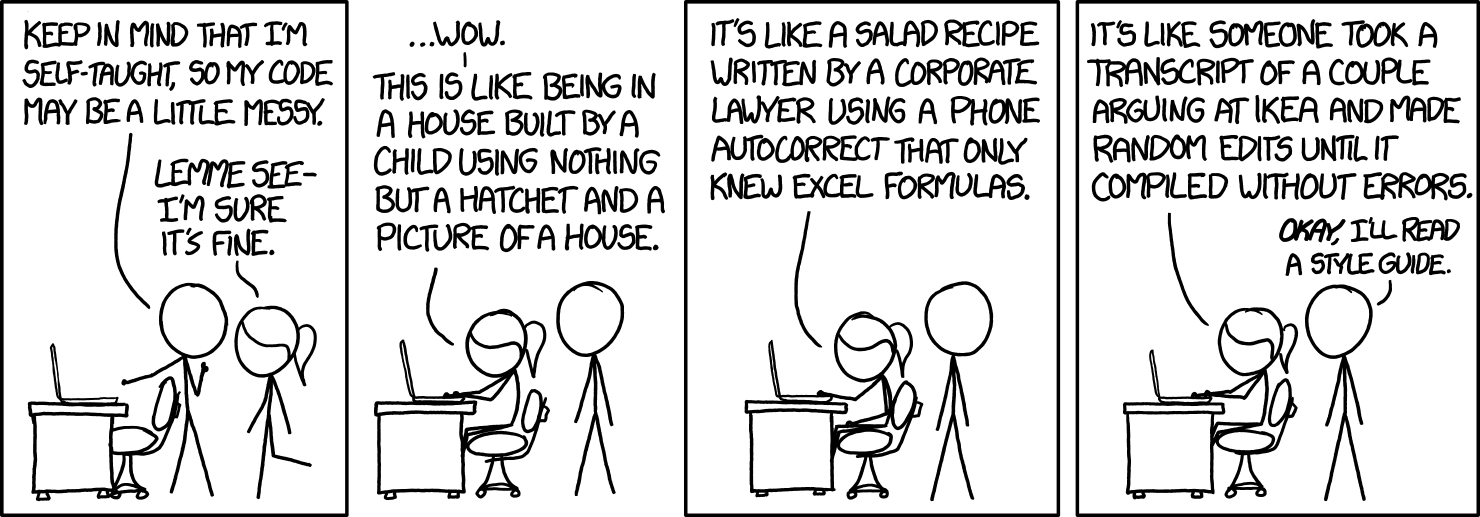
\includegraphics[width=\linewidth]{./gfx/xkcd-codeQuality}\\
	\emph{I honestly didn't think you could even USE emoji in variable names. Or that there were so many different crying ones.}

	\vspace{6pt}
	Source: \url{https://xkcd.com/1513/}
\end{center}
%
\end{frame}

% =========================================================================== %

\begin{frame}{Plan Your Code on Paper}
%
\begin{itemize}
\item Before you do anything: picture what you want to have
	\begin{itemize}
	\item Draw the look of your interfaces
	\item What does your input look like? File formats, numerical data, strings, ...
	\item What objects are you dealing with? Formulae, real-world-objects, ...
	\item What do you want to represent?
	\item Tell it to an (imaginary) particularly stupid person ... or to a rubber duck!
	\end{itemize}
\item Before writing first line of code: sketches
	\begin{itemize}
	\item Definitions (classes, in- and output of functions, data formats, ...)
	\item Data flow diagrams (\eg coordinates \thus\; \texttt{funcPotential} \thus\; container \thus\; sum)
	\item Conventions (rules for variable and function names, responsibilities)
	\end{itemize}
\item Then: do it all over again
	\begin{itemize}
	\item Identify repetitions \thus\; own functions or classes
	\item Parts that you looked up in your own sketch repeatedly? \thus\; redefine, unify
	\end{itemize}
\item GRIPS: Miniprojects BlackJack and SimCity
\end{itemize}
%
\end{frame}

% =========================================================================== %

\begin{frame}{Try to Predict the Future}
%
\begin{itemize}
\item When designing classes: are there obvious extensions to your modell?
	\begin{itemize}
	\item Don't implement them right away, but think of how you might go about that
	\item Additional parameters, generalizations
	\item Other means of output: on screen, into a file, into another file format, as a graph, ...
	\end{itemize}
\item What of your ideas now will you know in a month or a year from now?
	\begin{itemize}
	\item Plan and implement an easier to understand interface for your more complex components
	\end{itemize}
\item What of your planned features will you \emph{really} use?
	\begin{itemize}
	\item It's easy to get carried away and implement features that are never used, just because it's possible
	\item Keep your layout open to these expansions, but write them only if you need them
	\end{itemize}
\item \enquote{Separate constructing a system from using it}\\
	(Robert C. Martin, Clean Code)
\end{itemize}
%
\end{frame}

% =========================================================================== %

\begin{frame}{Encapsulation}
%
\begin{itemize}
\item Identify partial tasks of your goal (\emph{functional unit})
\item Each task more often than not has sub-tasks
\item Put the entire task into some encapsulation
	\begin{itemize}
	\item Simple: Functions
	\item More complex: Classes
	\item Still more complex: Modules
	\end{itemize}
\item The task as a whole can have its inner mechanics that is hidden from you later on
\item Thus you can forget about the whole while solving sub-problems or sub-sub-problems
\item Also: re-usable in later projects
\end{itemize}
%
\end{frame}

% =========================================================================== %

\begin{frame}{Don't Get Obsessed Over Runtime Efficiency}
%
\begin{itemize}
\item There are TONS of things to think about in each project
\item Optimization adds again TONS of food for thought
\item If you can handle all of that -- fine
\item Most likely, it's better to first write code that works and then think of what can be done better
\item Work in functional units
	\begin{itemize}
	\item Get unit to work
	\item Get unit to work \emph{fast}
	\item Write next unit
	\item Have a look at the interaction of both units
	\end{itemize}
\end{itemize}
%
\end{frame}

% =========================================================================== %

\begin{frame}{Test your Units in Well Defined Scenarios}
%
\begin{itemize}
\item For each functional unit, write a function that tests all the features
\item Intended way
\item Limit cases
\item Invalid input
	\begin{itemize}
	\item Safety features you did implement
	\item Invalid input you didn't think of yet
	\end{itemize}
\item This can double as a documentation
\end{itemize}
%
\end{frame}

% =========================================================================== %

\begin{frame}
%
\begin{columns}[T]
\column{.5\linewidth}
\begin{Large}
	{Write Lots and Lots of Code}
	\vspace{6pt}
\end{Large}
%
\begin{itemize}
\item Coding: Facing new problems every day
\item Hard to give good advice that is even applicable to many scenarios, let alone be true
\item Devellop a gut feeling ...
\item ... which you'll only gain over time
\item Read Code by others
\item Search Engine of your choice: plethora of blogs
\item Digest it bit by bit
\item With any luck, this class will give you some examples
\end{itemize}
%
\column{.5\linewidth}
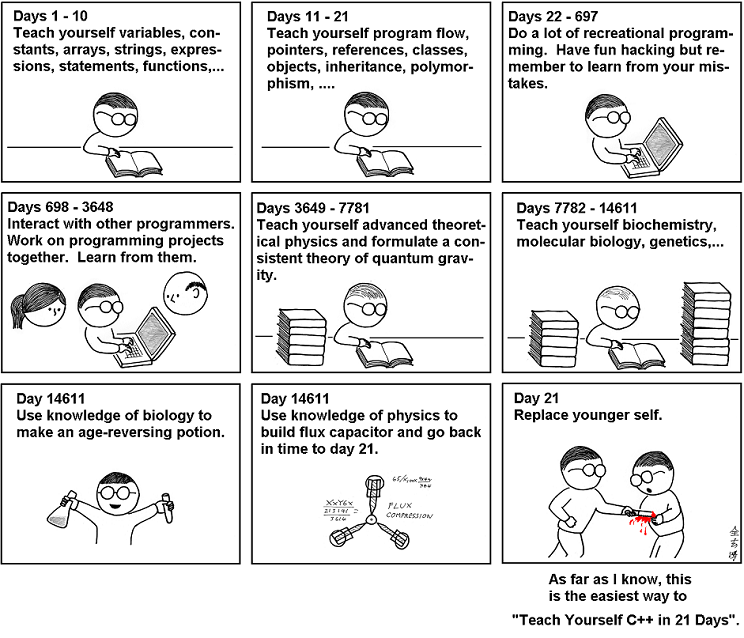
\includegraphics[width=\linewidth]{./gfx/agoose-249}
\url{https://abstrusegoose.com/249}
\end{columns}
%
\end{frame}